\subsection{Exploratory Search}
The search for information and (growing one's knowledge) is a built-in (property) in humans. Last few decades have transformed search and made it an everyday function. It wasn't until the late 1990's until web search services began offering quick access to information and traditional (thinking) about information retrieval had to be updated. Before the Web, information search services were used mainly by academics and information professionals. Small and motivated user base (prevented) search system manufacturers to focus on the user experience and the motivation to improve the user interface was (small). Traditional search systems were built on (query-results thinking) and as such, the query formulation was an essential stage of the search task []. Some studies have even evaluated systems, where the query results take days to return []. In such cases, the (user learns the system very slowly), since becoming a better user of such a system requires interaction with system and slow (query return) means slow learning.

Search system must be quick for other reasons too. Cognitive abilities restrict the searcher from running other tasks and starting sub-tasks in parallel with the original task []. That means the system should be simple and support user's (state of mind), not adding to the cognitive load already affecting the user. Whenever the user needs to (think on a higher level) it's possible the ‘flow' of the search task is lost. This so-called flow is a state of mind that the searcher has and having to set that aside might result in losing it.

\begin{figure}[htp] % t=top, h=here, b=bottom, p=separate page, !=place even if ugly
\caption{The classic information retrieval model. Based on \protect\cite{bates89}.}
\label{figure_classicIR}
\centering
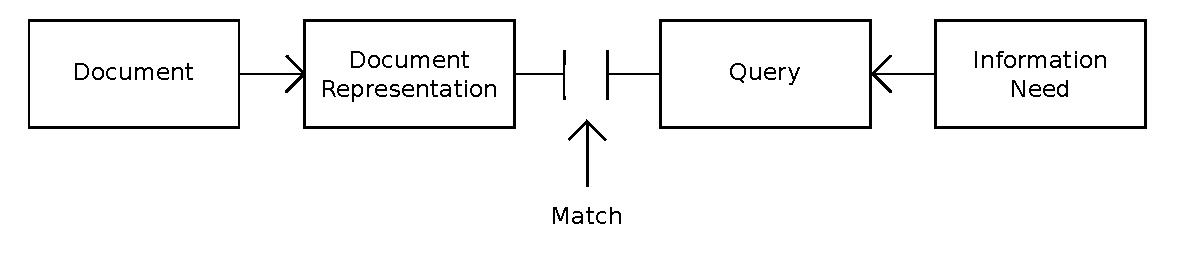
\includegraphics[scale=0.45]{figures/classicIR.pdf}
\end{figure}

The flow however, is not so important when the search task is simple. Let's think of a simple search task: a geography teacher has assigned a group of students to draw a poster about a European country and the group have chosen Denmark. They want to display some facts about the country in their poster, for example the population, land area and internet top-level domain. To retrieve these facts, a simple search with keyword Denmark will suffice.
The facts can be copied from Wikipedia or the official website of Denmark to the poster. This kind of lookup-based information retrieval model is described in Figure \ref{figure_classicIR}.
After finishing the poster, the group is given a new assignment.
Their second assignment is to write a play of a historical event that was of special importance for Denmark and then perform the play in front of the class.
This time, the information needed for completing the assignment is much more search task demands more time and is not as (easily definable) as in the previous assignment.
The students might start by reading the history of Denmark in the Wikipedia.
Along their exporation, they come upon different events and characters that have had an effect in Denmark's history.
With their now improved knowledge of Danish history, they need to decide which event they are to (display) in their play.
This requires collaboration within the group.
After decision on the event, the group needs to gather information on the people involved in the event. 
And if possible, they investigate what kind of clothes were used in the era the event took place in.
The tasks described (fit well in the strategy of) berry-picking. See Figure \ref{figure_bp}.

\begin{figure}[htp] % t=top, h=here, b=bottom, p=separate page, !=place even if ugly
\caption{An evolving berrypicking search. Based on \protect\cite{bates89}. From \protect\cite{march06}.}
\label{figure_bp}
\centering
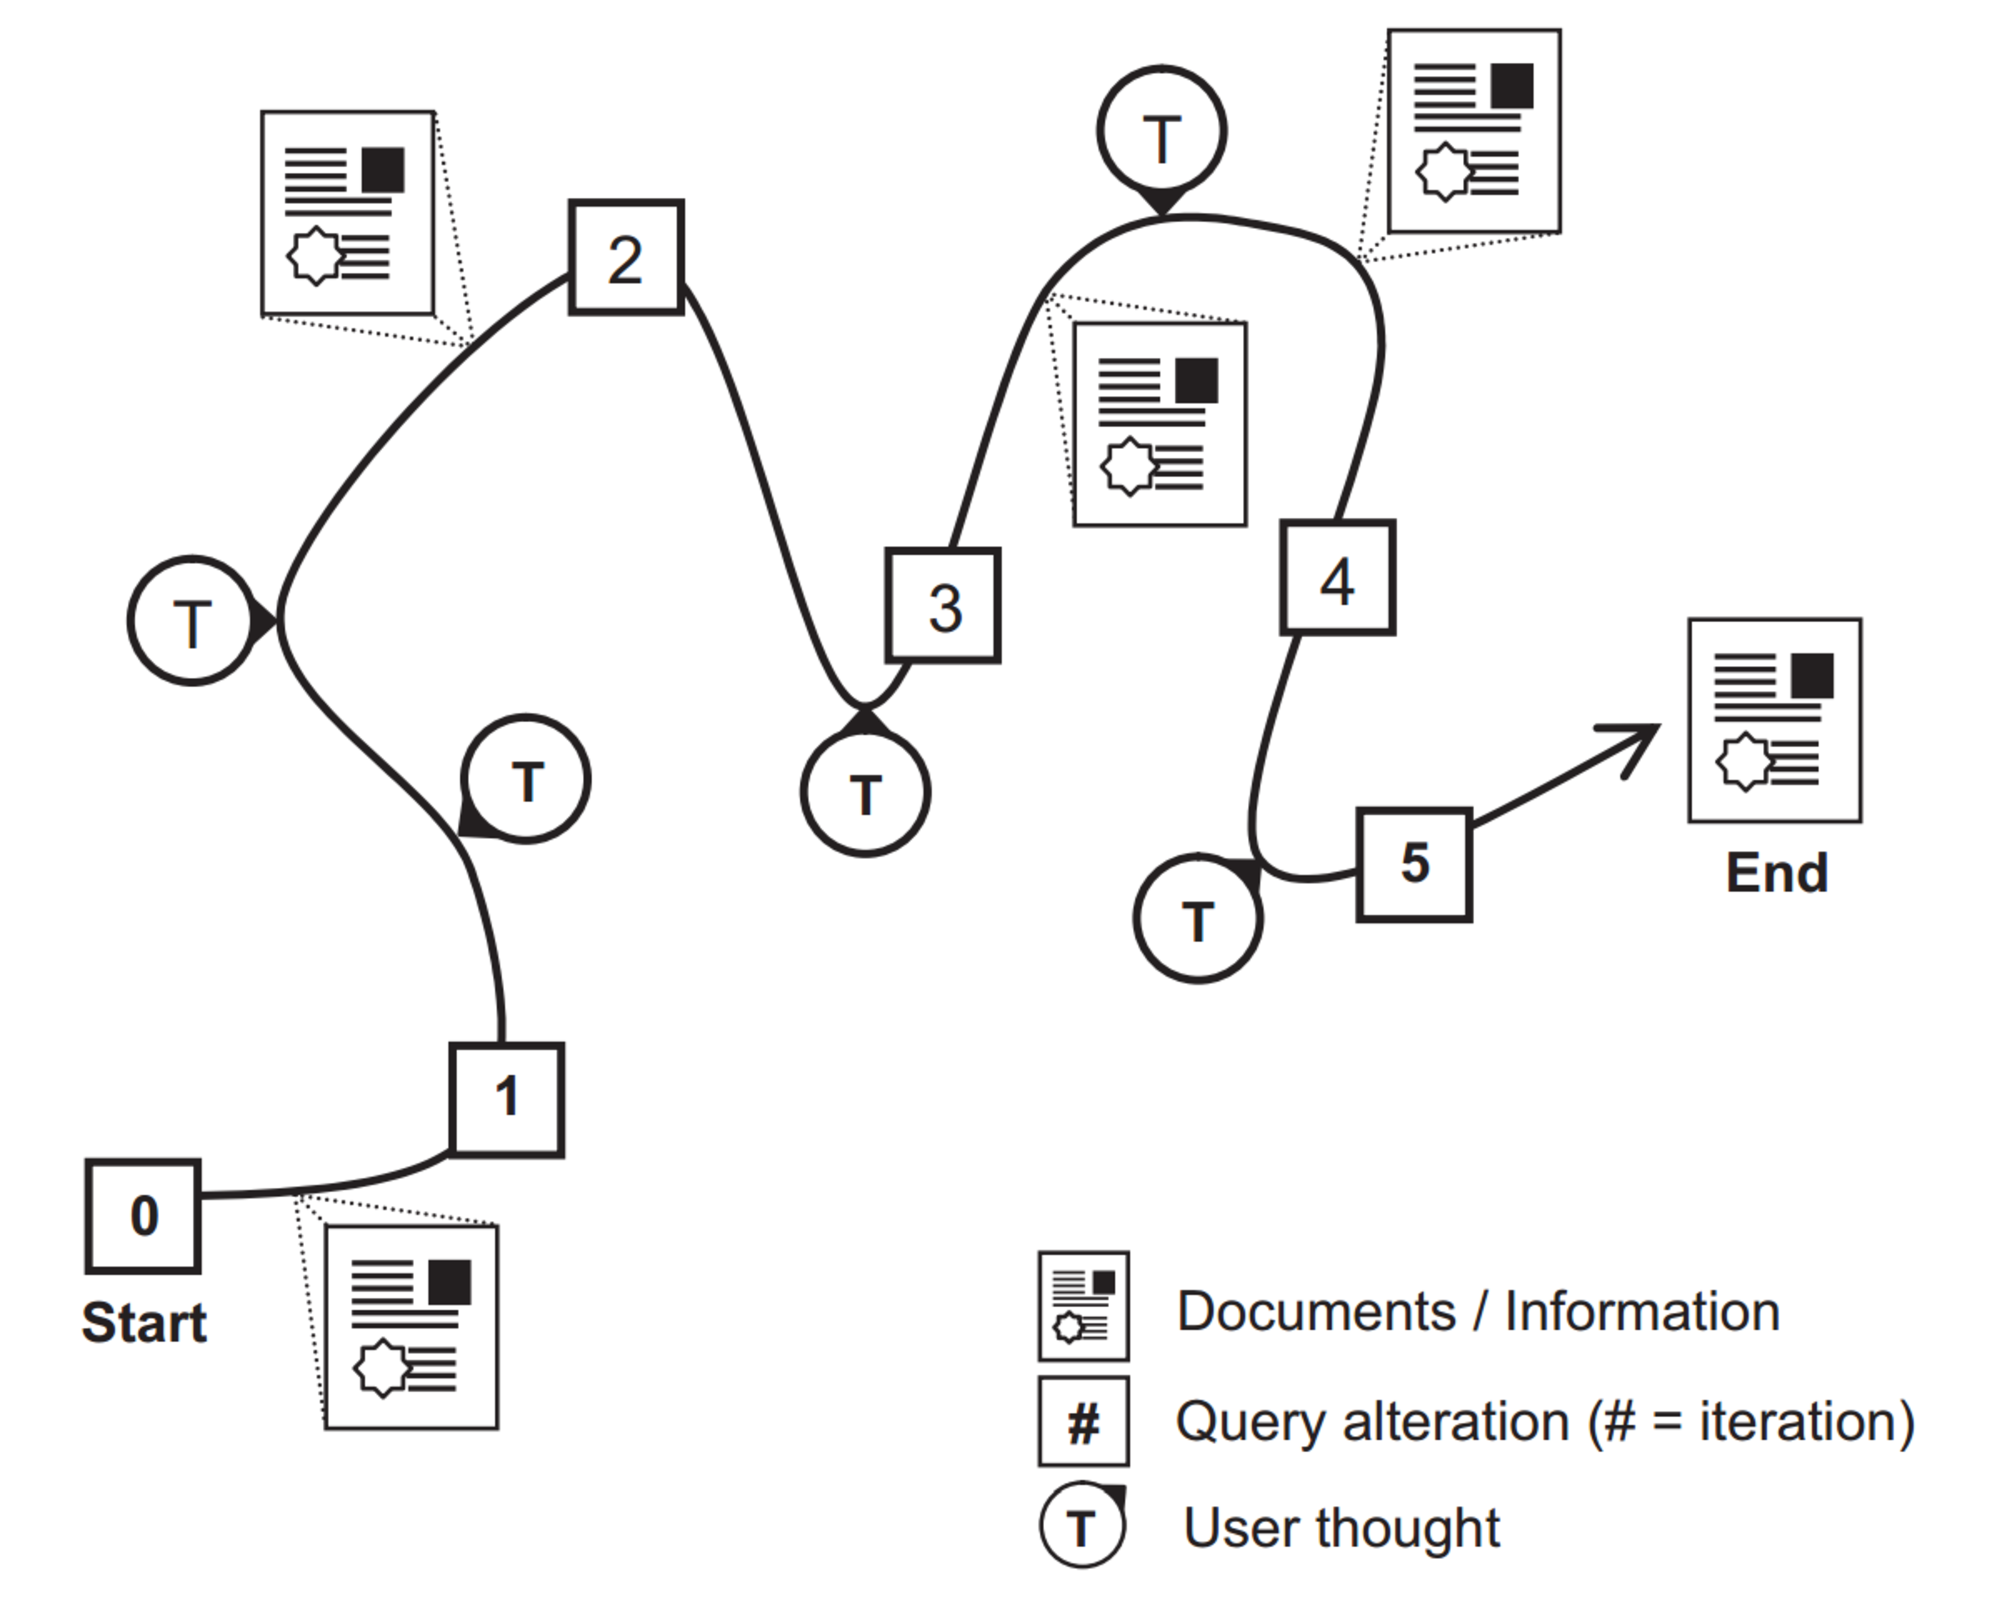
\includegraphics[scale=0.25]{figures/berrypicking.pdf}
\end{figure}

\begin{figure}[htp] % t=top, h=here, b=bottom, p=separate page, !=place even if ugly
\caption{Different search tasks are split into three overlapping search activities: \textit{lookup}, \textit{learn} and \textit{investigate}. Based on \protect\cite{march06}.}
\label{figure_3clouds}
\centering
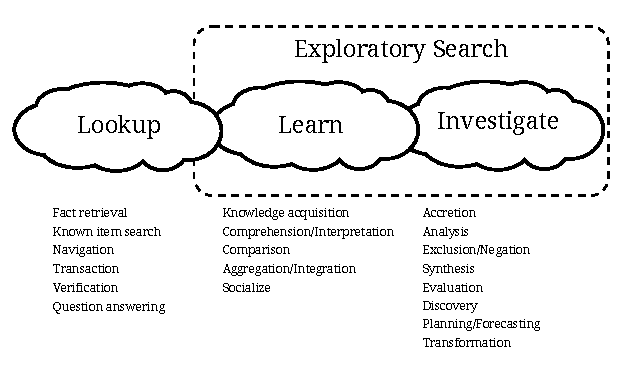
\includegraphics[scale=0.8]{figures/3clouds2.pdf}
\end{figure}

Introduction to exploratory search. See Figure \ref{figure_3clouds}.
\cite{march06}, \cite{white09}, \cite{tvaro11}

The user interface of an exploratory search system should be designed to fulfill the needs of most of its users. More information on what works and doesn't work can usually be collected from system evaluations.

However, evaluating exploratory search systems is difficult, because users have different starting positions. Their knowledge of the domain varies, they are interested in different aspects of the topic and they have previously encountered different information. \cite{kules08}

Exploratory search and iterative search differ. See Figure \ref{figure_IterativeVsExploratory}.

\begin{figure}[htp] % t=top, h=here, b=bottom, p=separate page, !=place even if ugly
\caption{They differ. From \protect\cite{white09}.}
\label{figure_IterativeVsExploratory}
\centering
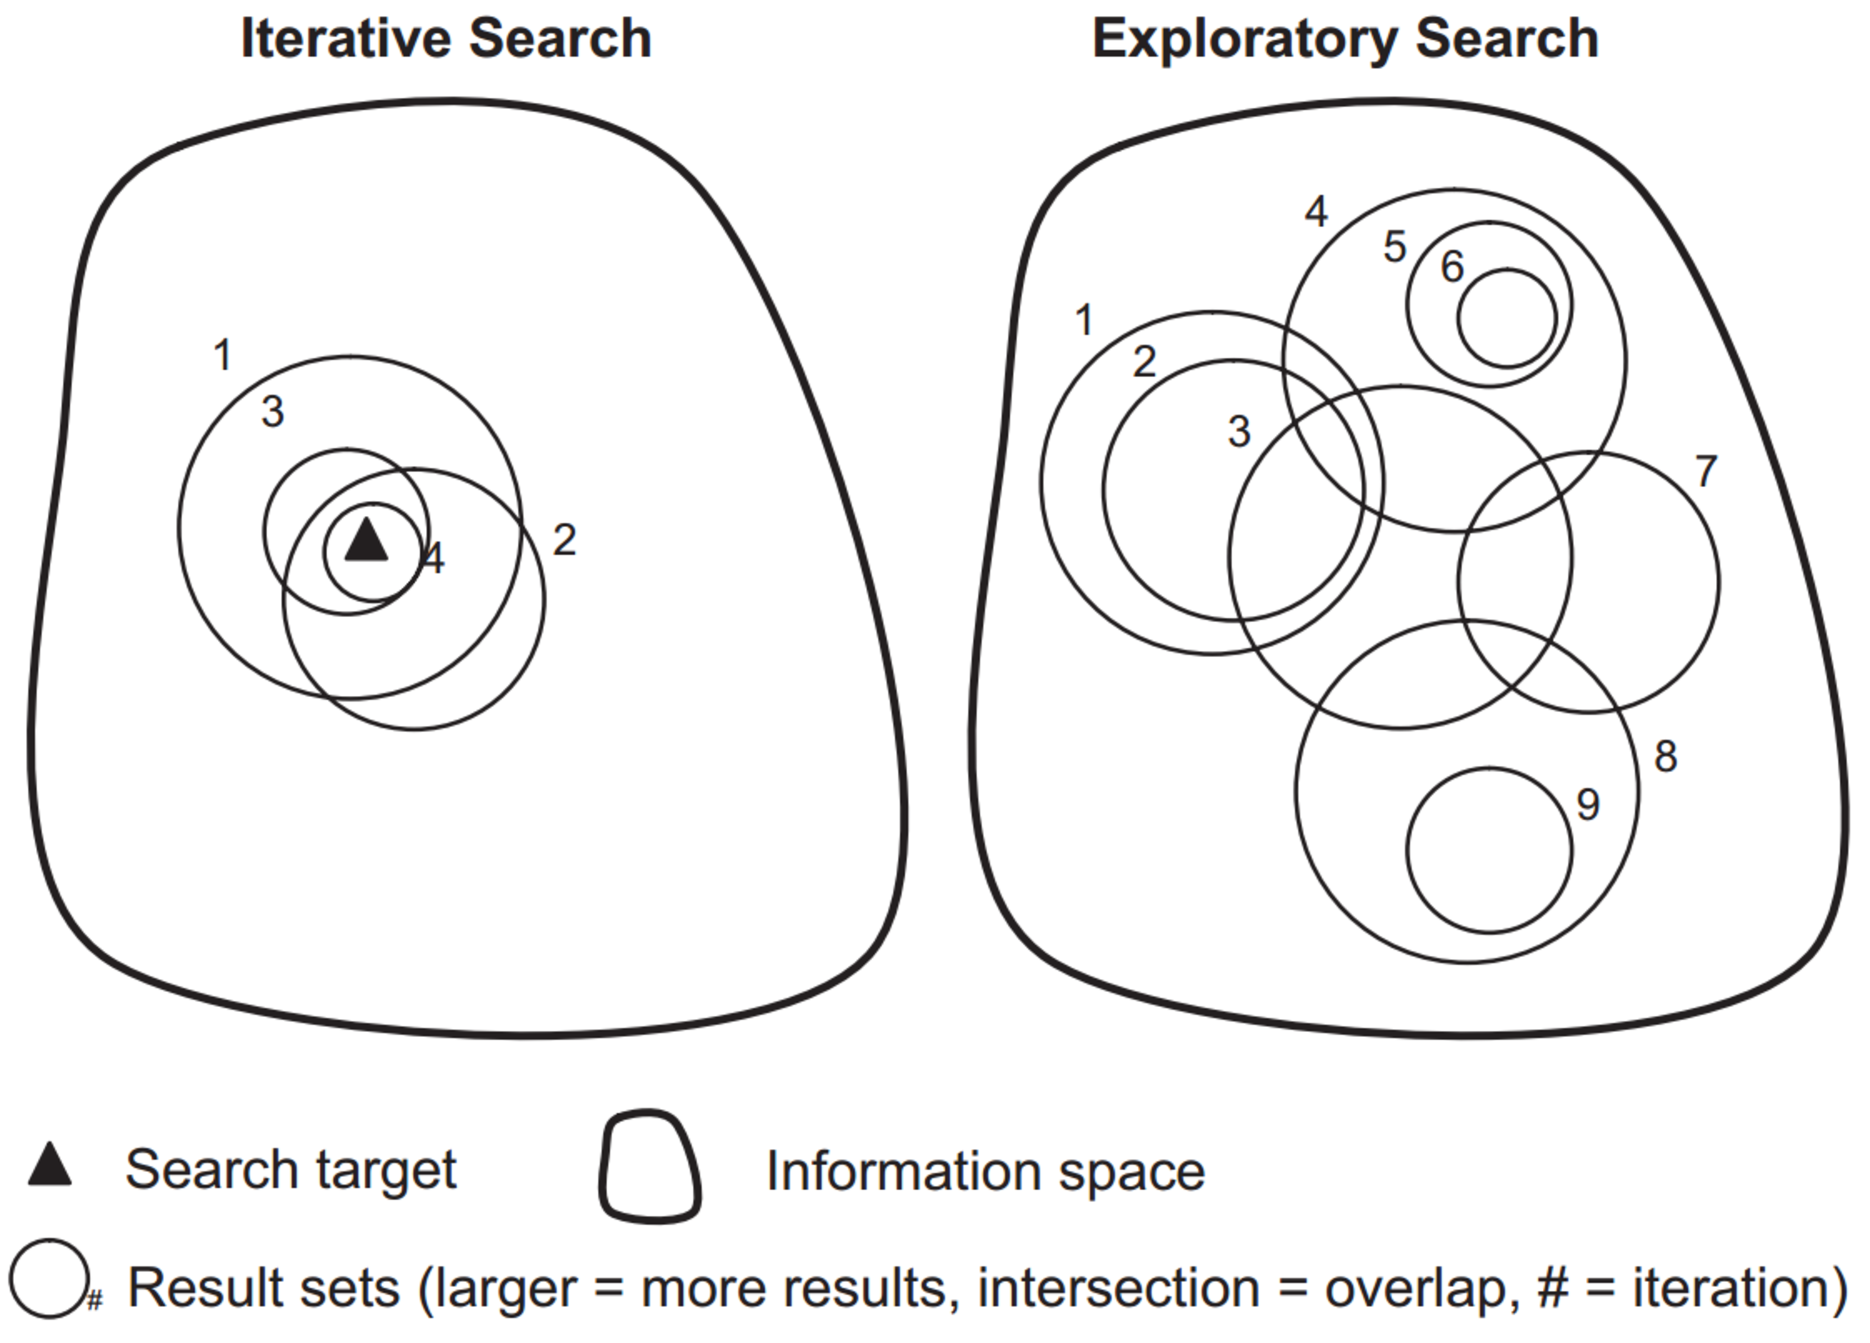
\includegraphics[scale=0.25]{figures/IterativeSearch_vs_ExploratorySearch.pdf}
\end{figure}

Exploratory search tasks can be characterized as either learning oriented or investigative  and they have common aspects like uncertainty, ambiguity and discovery distinguishing them from look-up oriented tasks \cite{kules09}.

